
    \documentclass[11pt]{scrartcl}
    \usepackage{textcomp}
    \usepackage{gensymb}
    \usepackage{graphicx}
    \usepackage{grffile} %required because there are multiple dot characters in my file names
    \usepackage{booktabs}
    \usepackage[letterpaper, margin=1in]{geometry}
    \usepackage{booktabs}
    \usepackage{multirow}

    \usepackage[unicode=true,pdfusetitle,
    bookmarks=true,bookmarksnumbered=false,bookmarksopen=false,
    breaklinks=true,pdfborder={0 0 0},pdfborderstyle={},backref=false,colorlinks=true]
    {hyperref}
    \hypersetup{linkcolor=blue,citecolor=blue,urlcolor=blue}

    \titlehead{\centering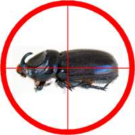
\includegraphics[width=0.75in]{static/images/crb_logo.png}\\
    University of Guam Coconut Rhinoceros Beetle Biological Control Project\\
    Generated by bioassay-report-generator.ipynb v.2019-10-29\\
    \url{https://github.com/aubreymoore/rearing3}}

    \title{Bioassay Report: V23BperOS}

    \author{Aubrey Moore and James J. Grasela\\University of Guam Coconut Rhinoceros Beetle Biocontrol Project}
    \begin{document}
    \begin{titlepage}
        \maketitle
        \begin{center}
            \url{https://github.com/aubreymoore/rearing3/raw/master/bioassay-V23BperOS.pdf}
        \end{center}
        \tableofcontents
    \end{titlepage}
    
    
% Please add the following required packages to your document preamble:
% \usepackage{booktabs}
% \usepackage{multirow}
\begin{table}[]
	\begin{tabular}{@{}lcccccccl@{}}
		\toprule
		\textbf{\begin{tabular}[c]{@{}l@{}}OrNV\\ isolate\end{tabular}} & \textbf{bioassay} & \textbf{method} & \textbf{beetles} & \textbf{replicates} & \textbf{\begin{tabular}[c]{@{}c@{}}virus\\ mortality\end{tabular}} & \textbf{p} & \textbf{\begin{tabular}[c]{@{}c@{}}heat\\ inactivated\\ virus\\ mortality\end{tabular}} & \multicolumn{1}{c}{\textbf{p}} \\ \midrule
		DUG42 & DUG42 & injection & 30 & 2 & 40\% & 0.65 & 40\% & 0.65 \\
		\midrule
		\multirow{2}{*}{MALB} & MALB & injection & 30 & 2 & 50\% & 0.37 & 0\% & 1.00 \\
		& MALBperOS & per os & 13 & 1 & -60\% & 1.00 & 20\% & 1.00 \\
		\midrule
		\multirow{2}{*}{PNG} & PNG & injection & 81 & 4 & \textbf{90\%} & \textbf{0.00} & 5\% & 1.00 \\
		& PNGperOS & per os & 21 & 1 & 0\% & 1.00 & 0\% & 1.00 \\
		\midrule
		\multirow{4}{*}{V23B} & V23B & injection & 66 & 4 & \textbf{88\%} & \textbf{0.00} & 0\% & 1.00 \\
		& V23BperOS & per os & 32 & 2 & 80\% & 0.07 & 20\% & 0.69 \\
		& V23-large\_bioassay & per os & 53 & 1 & \textbf{42\%} & \textbf{0.00} & - & - \\
		& V23\_perOSIN & per os & 16 & 1 & 60\% & 0.06 & - & - \\ 
		\bottomrule 
	\end{tabular}
\end{table}
    
    \clearpage
    \section{Summary}

    \begin{table}[h!]
        \centering
        \caption{Bioassay summary.}
        \begin{tabular}{lllllr}
\toprule
{} & bioassay\_name & date\_start\_bioassay & date\_end\_bioassay & bioassay\_treatment &  N \\
\midrule
0 &   V23BperOS-1 &          2019-03-05 &        2019-04-05 &            control &  6 \\
1 &   V23BperOS-1 &          2019-03-05 &        2019-04-05 &   heat inactivated &  5 \\
2 &   V23BperOS-1 &          2019-03-05 &        2019-04-05 &              virus &  5 \\
3 &   V23BperOS-2 &          2019-04-12 &        2019-05-10 &            control &  6 \\
4 &   V23BperOS-2 &          2019-04-12 &        2019-05-10 &   heat inactivated &  5 \\
5 &   V23BperOS-2 &          2019-04-12 &        2019-05-10 &              virus &  5 \\
\bottomrule
\end{tabular}

    \end{table}

    Fifteen adult beetles maintained for more than 2 weeks to observe possible contamination from green muscardine fungus infection were employed in a preliminary test to determine the susceptibility of adult beetle to infection by virus \textbf{V23 B} isolate (Solomon Islands). Each of 5 beetles (5/treatment) were orally fed 10 {\micro}l of a virus + 30\% sucrose mixture with a sterile pipette tip. Adults were then placed in clean glass mason jars (bleach-treated) with a piece of banana added for food. Beetles were incubated at 30{\celsius} and 80\% RH in a Percival incubator. All beetles will be monitored daily to observe any possible signs of infection.
    
   \clearpage
   \section{Mortality}

   \begin{table}[h!]
       \centering
       \caption{Mortality summary.}
       \begin{tabular}{llrrrrr}
\toprule
{} & bioassay\_treatment &  ntotal &  ndead &  mortality &  adjusted\_mortality &  significance \\
\midrule
0 &            control &      12 &      6 &        0.5 &                 0.0 &      1.000000 \\
1 &   heat inactivated &      10 &      4 &        0.4 &                -0.2 &      0.691355 \\
2 &              virus &      10 &      9 &        0.9 &                 0.8 &      0.074303 \\
\bottomrule
\end{tabular}

   \end{table}

   \begin{center}
        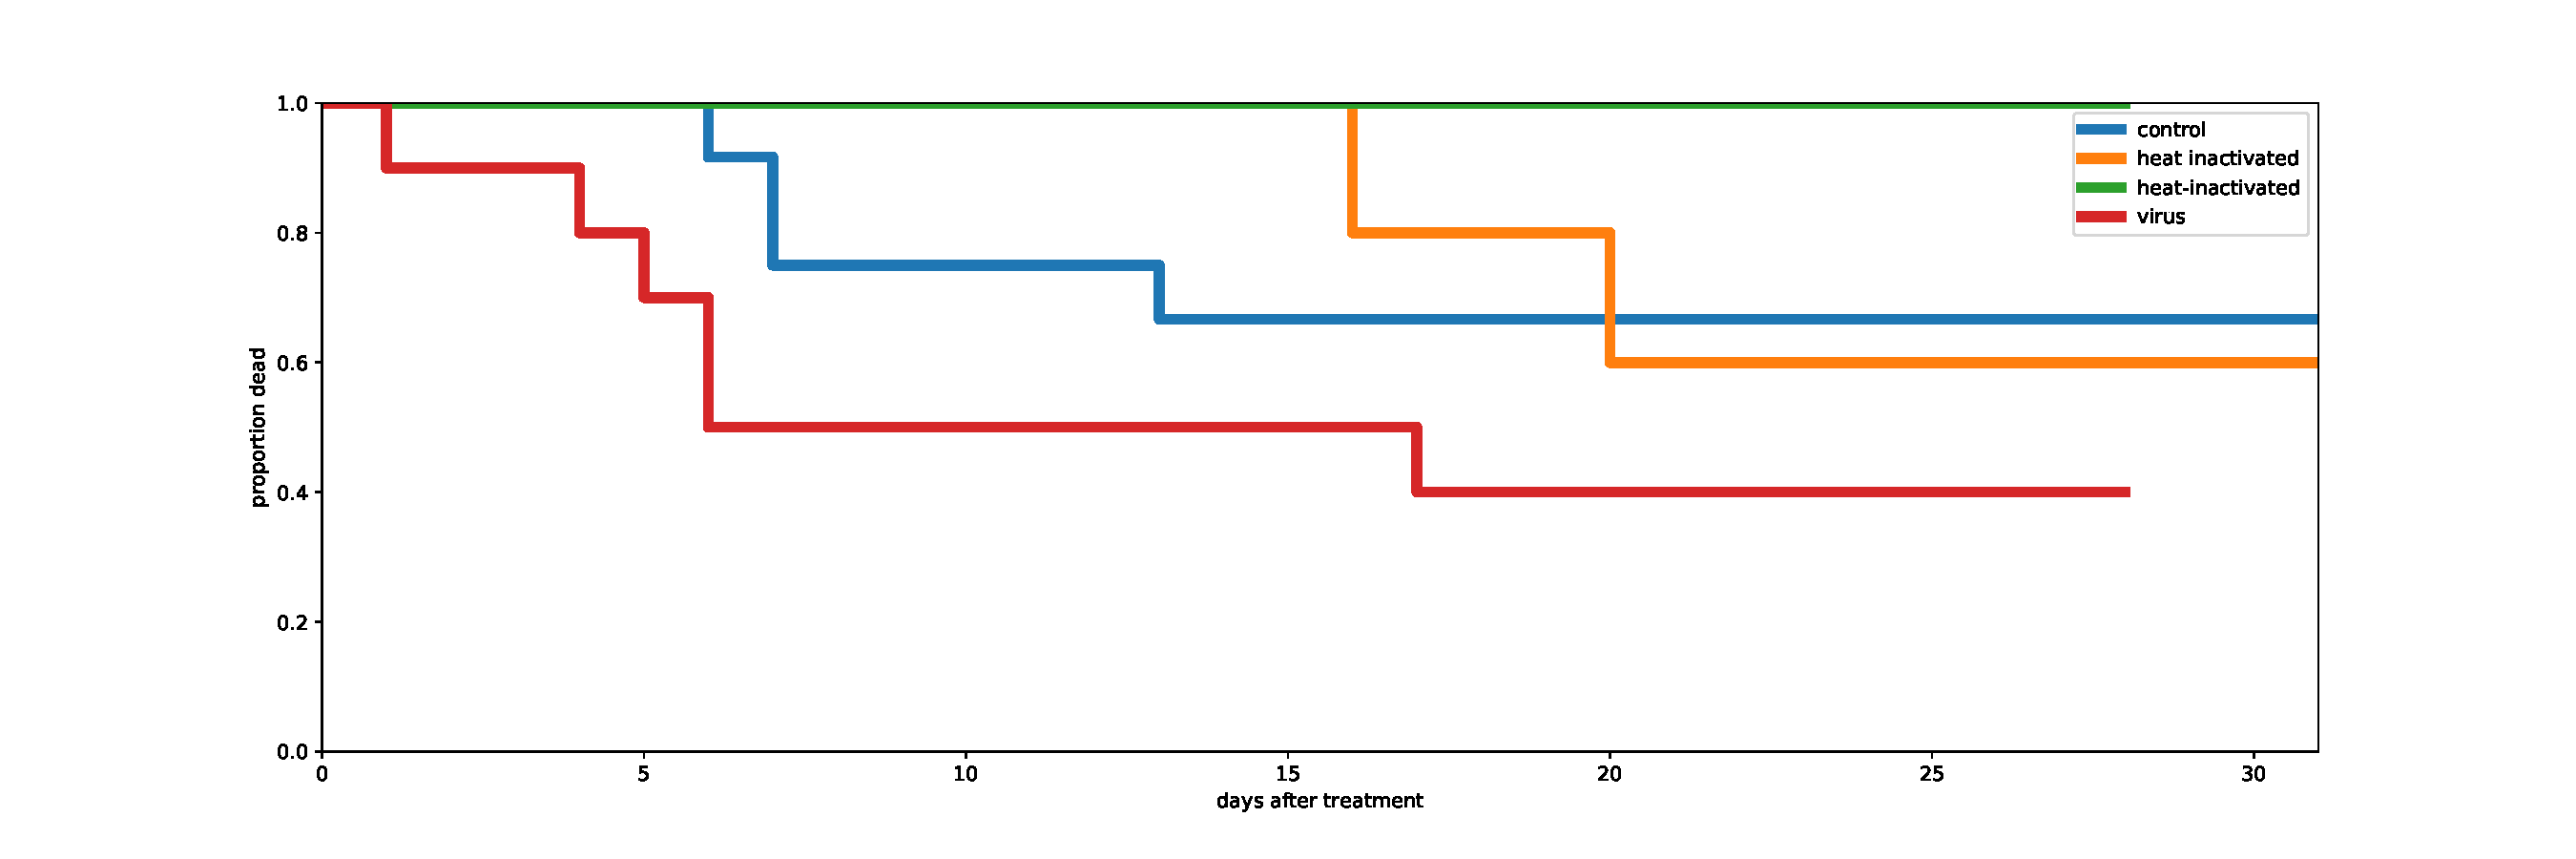
\includegraphics[width=\textwidth]{survivorshipfig.pdf}
   \end{center}


   
       \begin{table}[h!]
       \centering
       \caption{Pairwise differences among mortality curves.}
   \begin{tabular}{llrr}
\toprule
                 &       &  test\_statistic &         p \\
\midrule
control & heat inactivated &        0.350703 &  0.553716 \\
                 & virus &        4.076804 &  0.043476 \\
heat inactivated & virus &        5.842978 &  0.015639 \\
\bottomrule
\end{tabular}
\end{table} 
   
    \clearpage
    \section{Change in Mass}

    \begin{center}
         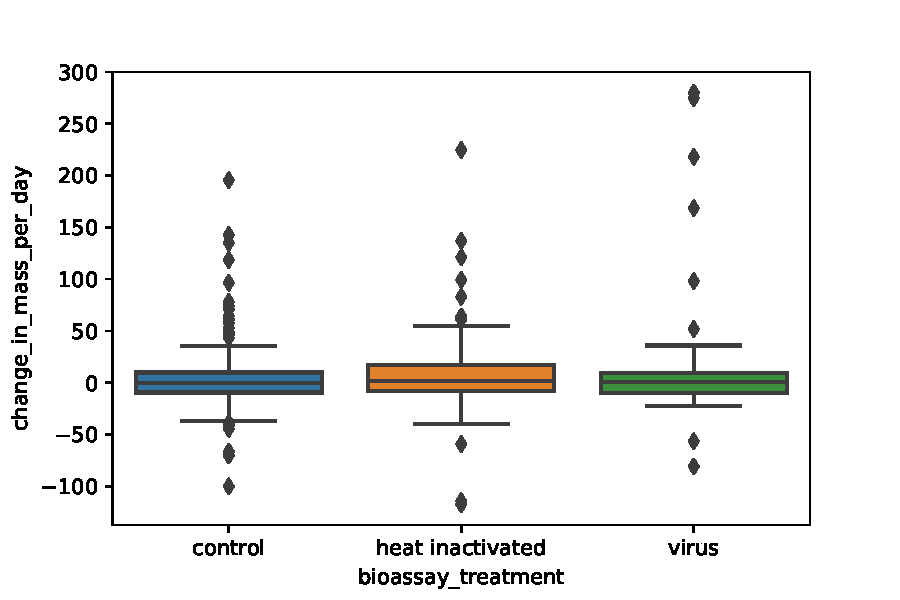
\includegraphics[width=\textwidth]{bp.pdf}
    \end{center}

    \begin{table}[h!]
        \centering
        \caption{Results of pairwise significance tests for differences in change in mass.}
    \begin{tabular}{lrrr}
\toprule
{} &   control &  heat inactivated &     virus \\
\midrule
control          & -1.000000 &          0.740696 &  0.245085 \\
heat inactivated &  0.740696 &         -1.000000 &  0.157019 \\
virus            &  0.245085 &          0.157019 & -1.000000 \\
\bottomrule
\end{tabular}

    \end{table}
    \end{document}